\subsection{MEX 0-1b: Three-Point fracture toughness test, Opalinus Claystone}

\subsubsection*{CAU Kiel}

The experimental results of the three-Point fracture toughness test on the Opalinus Claystone samples are uploaded to the IfG (Kiel) NextCloud server. The data is accessible through the following link:\\
\hyperlink{https://nextcloud.ifg.uni-kiel.de/index.php/s/pJxp2eNEJb6PfiS}{https://nextcloud.ifg.uni-kiel.de/index.php/s/pJxp2eNEJb6PfiS}\\

The data set, which includes the time, applied force ($N$) and the displacement of the sample at the loading point ($mm$), is provided in a *.txt file. The crack mouth opening displacement (CMOD), which is determined from the image processing technique (section \ref {sec:Fracture_Toughness_Exp}), is given in a *.xlsx file. The data includes the time and the calculated CMOD (mm). 

The required LEM code and the input variables of the three-Point fracture toughness test on the Opalinus Claystone samples are uploaded to the IfG (Kiel) NextCloud server. The data is accessible through the following link:\\
\hyperlink{https://nextcloud.ifg.uni-kiel.de/index.php/s/ZBFN2rSZ99kPY9M}{https://nextcloud.ifg.uni-kiel.de/index.php/s/ZBFN2rSZ99kPY9M}\\

The uploaded protected MATLAB file in a *.p format requires a MATLAB version with a built-in Voronoi Tessellation and Delaunay Triangulation functions. The input variables are prepared in two different files for a parallel and perpendicular embedded layer orientations. Figure \ref{fig:Amir_ME1_LEM_Claystone_Data} shows the comparison between the experimental and numerical data as described in section \ref {sec:mex01b}.

\begin{figure}[!ht]
\centering
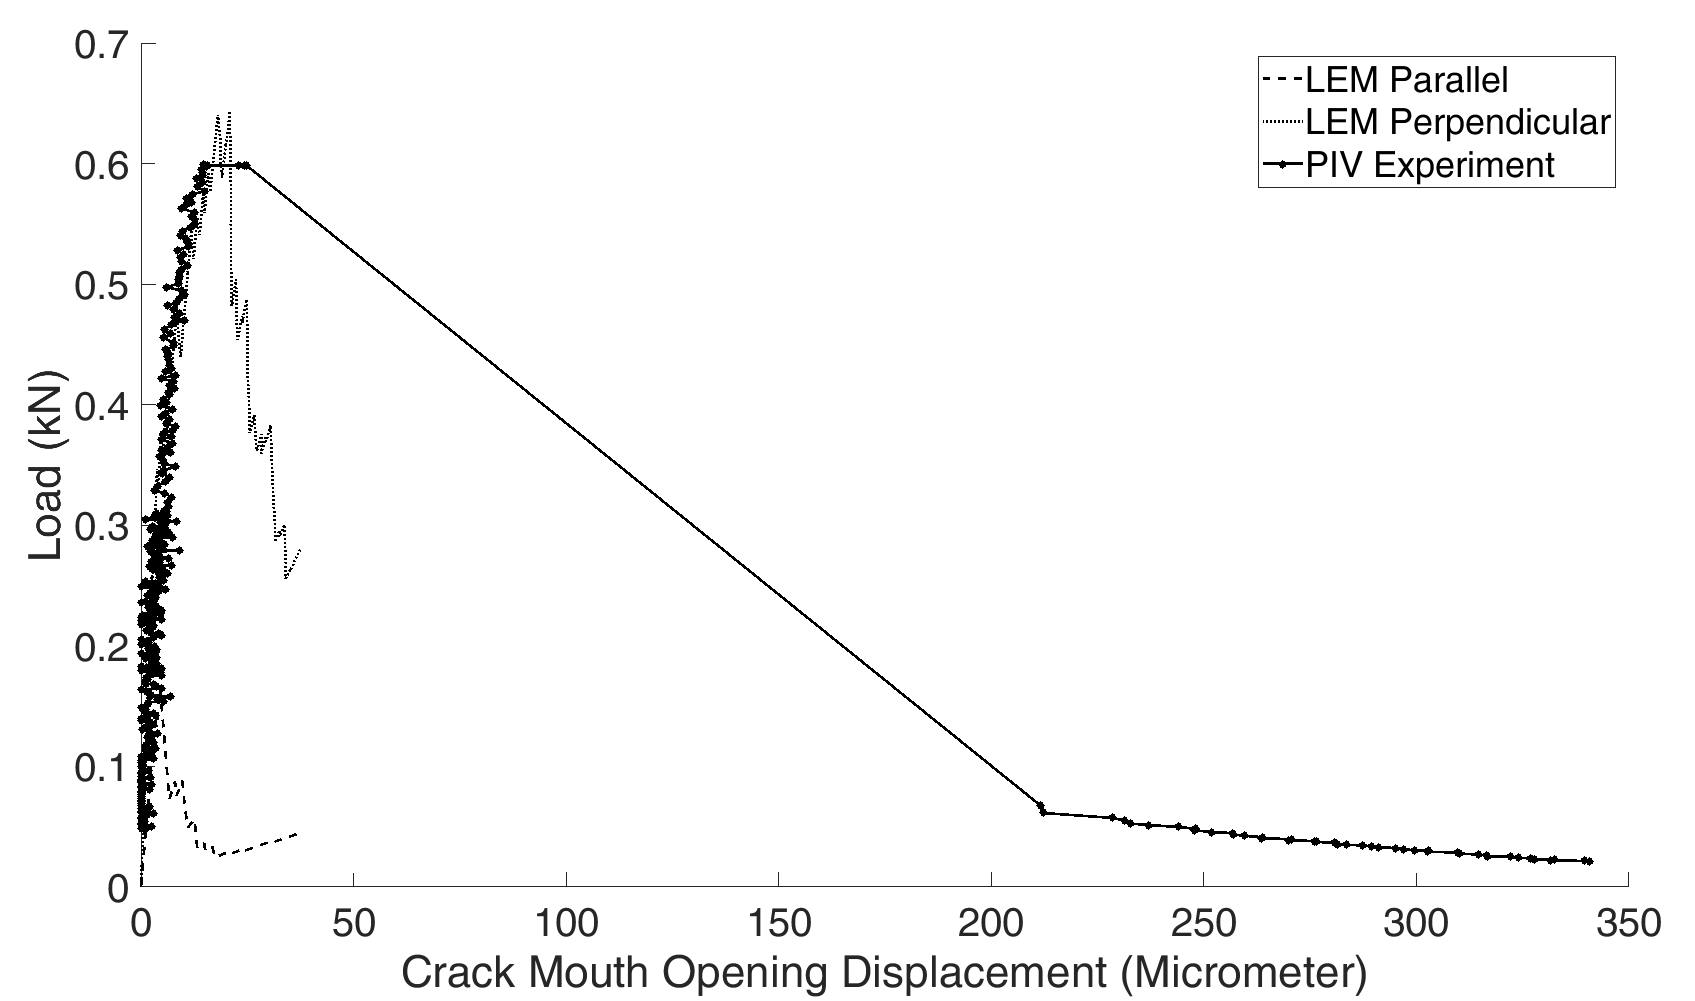
\includegraphics[width=0.75\textwidth]{figures/Amir_ME1_LEM_Claystone_Data.png}
\caption{The load vs. crack mouth opening displacement (CMOD) response of the Opalinus claystone}
\label{fig:Amir_ME1_LEM_Claystone_Data}
\end{figure}

\begin{table}[!ht]
\caption{MEX 0-1b: Bending fracture test, Opalinus Claystone}
\label{tab:dms-mex0-1b}
\small
\begin{tabular}{R{3cm}|L{7cm}}
\hline
%
Data label & GeomInt | CAU |  Bending fracture test, Opalinus claystone \\
URI &  https://nextcloud.ifg.uni-kiel.de/index.php/s/pJxp2eNEJb6PfiS (Experiments), https://nextcloud.ifg.uni-kiel.de/index.php/s/ZBFN2rSZ99kPY9M (Numerics)\\
Subject  &  Bending fracture test, Opalinus claystone\\
Type of data  &  Experimental data, executable MATLAB P-file, input parameters\\
Dataquality  &  quality assured data \\
Status of data  &  unprocessed data\\
Dataformat  & txt, xlsx, MATLAB executable P-file\\
Creators  &  Kiel University, Institute of Geomechanics and Geotechnics, Ludewig-Meyn-Stra\ss e 10, 24118, Kiel\\
Source/Origin & In-house code \\
Publisher  &  Kiel University, Institute of Geomechanics and Geotechnics, Ludewig-Meyn-Stra\ss e 10, 24118, Kiel \\
Rights holders &  Kiel University, Institute of Geomechanics and Geotechnics, Ludewig-Meyn-Stra\ss e 10, 24118, Kiel \\
Contributors &   Kiel University, Institute of Geomechanics and Geotechnics: Amir Shoarian Sattari, Frank Wuttke\\
Time or Period of creation &  2018-2019\\
Language of the content &  English\\
Update policy &  stored data is final\\
Access permissions & full access\\
%
\hline
\end{tabular}
\end{table}

\subsubsection*{UFZ}
The input files for OGS, which were used to simulate the three point bending test performed on the orthogonal and parallel laminations of Opalinus claystone samples, have been uploaded.
The files include the unstructured finite element mesh files in vtu format and OGS input files in xml format.
Also in the mesh files, the material properties are defined per element. 
Particularly for the orthogonal and the parallel Lamentations in the samples are represented through a contrast in the fracture toughness in the samples and can be found in the mesh files.
The load and crack mouth opening displacment computed from the simulations are shown in~\ref{fig:Keita_ME1_VPF_Claystone} as described in section \ref {sec:mex01b}.

\begin{figure}[!ht]
\centering
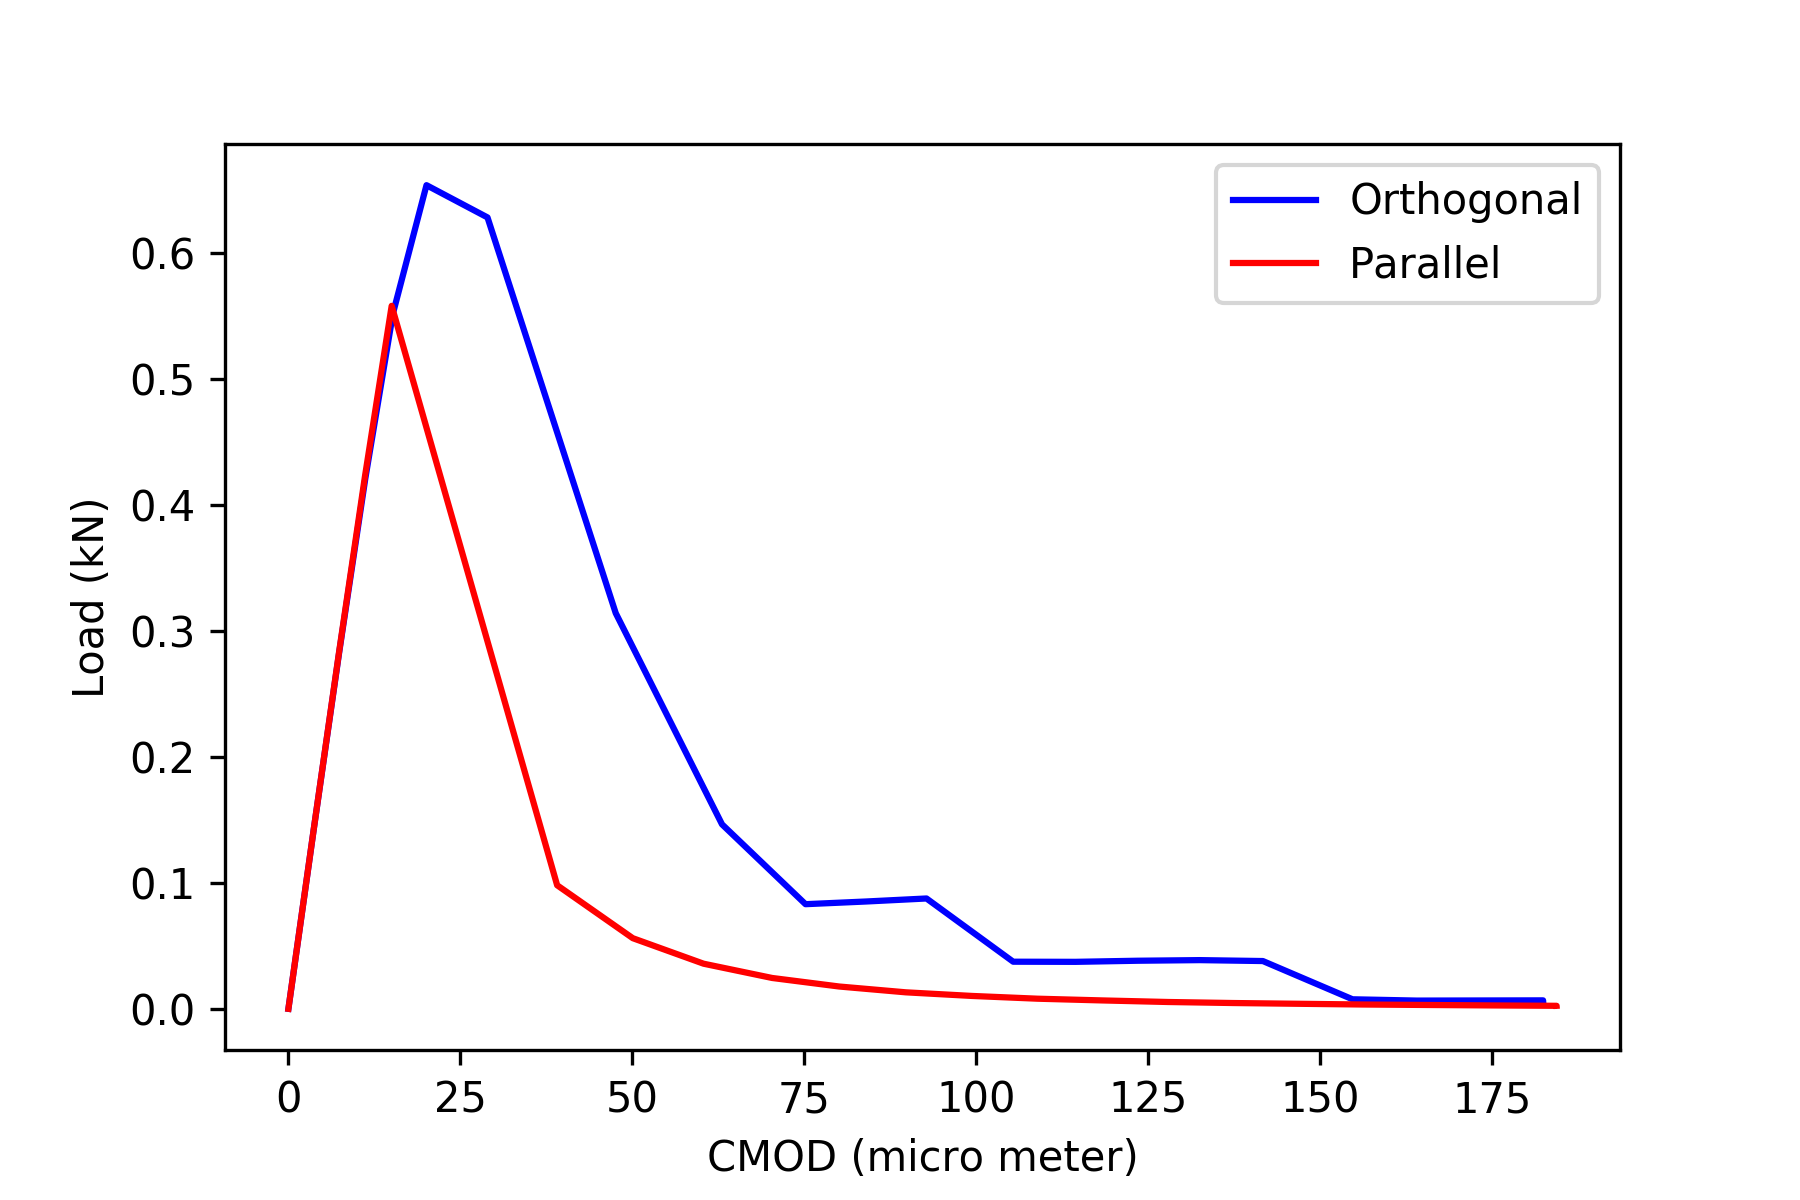
\includegraphics[width=0.75\textwidth]{figures/VPF_ME1_ex_NF_CMOD.png}
\caption{The load vs. crack mouth opening displacement (CMOD) response simulations for orhtogonal and parallel lamination by VPF.}
\label{fig:Keita_ME1_VPF_Claystone}
\end{figure}